\documentclass{vs-thesis}
\setdefaultlanguage{english} % english or german 

% This package is only used in the demo and should be removed for the actual thesis.

% todo notes. (hint: remove for final version)
\usepackage[backgroundcolor=white,linecolor=red,bordercolor=red,textsize=footnotesize]{todonotes}
\usepackage{pdfpages}

% Loads bibliography for citations.
\addbibresource{bibliography.bib}

% Define necessary metadata here
\title{Comparing Different Vehicle Architectures Based On Attack Path Analysis}
\thesistype{Bachelor Thesis}
\titlegraphic{titleimage.jpg}
\submissiondate{\today}

\author{Emilija Kastratović}
\studentnumber{1052407}
\internalid{VS-2019-B18}
\place{Ulm}

\examiners{
    Prof.\@~Dr.\,rer.\,nat.\@~Frank Kargl
}
\supervisors{M.Sc.\@~Michael Wolf}

\institution{
    Institute of Distributed Systems\\
    Faculty of Engineering, Computer Science and Psychology\\
    Ulm University}

\license{\ccby}


\usepackage[acronym,toc,automake]{glossaries}
\loadglsentries{glossary.tex}
\makeglossaries


\begin{document}

\frontmatter
\maketitle
\makeabstract
\tableofcontents

\mainmatter
%************************************************
\chapter{Introduction}
\label{chp:introduction}
%************************************************

\section{Research field: Cybersecurity of vehicular networks}
\label{sec:field}

Modern vehicles are becoming increasingly reliant on technology, with a wide range of systems and components being connected to the internet and each other. 
This includes everything from infotainment systems and navigation to advanced driver assistance systems and autonomous driving features.
ISO 26262 describes these so-called "\gls{e/e} Systems" as systems that consist of electrical and electronic elements and components such as \gls{ecu}s, sensors, actuators, connections, and communication systems like \gls{can}, Ethernet, and Bluetooth \cite{iso26262}.
As these technologies become more important, the need for strong cybersecurity measures becomes increasingly important. 
Hackers and cybercriminals are constantly finding new ways to exploit vulnerabilities in these systems, which can have serious consequences. 
This includes their safety, privacy, finances, and operational viability. Ensuring the safety and security of connected vehicles is crucial to the success of the emerging world of connected and autonomous transportation.
\\

The internal vehicular network architecture plays a crucial role in the overall cybersecurity of a modern vehicle because it determines how different vehicle systems and components are connected and communicate. 
\gls{attack path}s play an important role in vehicle networks and security because they help companies understand the specific routes or methods that a malicious actor might use to attack a vehicle's systems or networks. 
For example, companies can implement appropriate security measures to prevent these attacks by understanding the attack paths that might be used to gain unauthorized access to a vehicle's systems. 
These include encryption, authentication protocols, and firewall systems to protect against cyber threats. 
A well-designed internal vehicular network architecture can help minimize cyberattack risk. 
As the number of systems and components that are connected to the internet and each other increases, so too does the complexity of the internal vehicular network architecture. 
This can make it more challenging to design and implement effective cybersecurity measures, as more potential points of vulnerability need to be addressed. 
Therefore, companies developing connected and autonomous vehicles need to prioritize cybersecurity in designing their internal vehicular network architecture, 
which can help to ensure the safety and security of the vehicle, as well as protect the privacy and personal data of drivers and passengers,
\\

Methods for security testing, like penetration testing, are often carried out in the late stages of development, which can lead to the discovery of vulnerabilities at a time when it is more difficult and costly to address.
Additionally, pentesting is considered to be a skill-based activity that is still carried out manually.
It requires a high level of expertise and experience with other cybersecurity tools and techniques. 
A \gls{tara} is a crucial element for security assessment. 
Companies perform a TARA during the development process to identify and prioritize potential risks and to implement controls or countermeasures to reduce or mitigate those risks to an acceptable level. 
The increased complexity of modern vehicles and the arduous nature of the state-of-the-art security testing methods make it more unfeasible for companies to conduct security assessment testing as is done now. 
Thus, a need for an automated tool that can help resolve this issue and couple to the TARA process is apparent. 

TODO: Was ich in der arbeit mache und herausgefunden habe

\section{Thesis Questions}
\label{sec:thesis-questions}

The questions this thesis will answer include:

\begin{itemize}
    \item How can different E/E architectures be rated based on attack paths?
    \item How secure is the given vehicular network architecture?
    \item What architectural approach makes a network safer than others?
    \begin{itemize}
        \item How do small changes in network positioning affect the network security overall?
        \item How do simple and more branched out networks compare in terms of security?
    \end{itemize}
\end{itemize}



\section{Background and Motivation}
\label{sec:background}

TODO: kann weg
As a computer science student with a passion for cybersecurity and a focus on cybersecurity in my studies, I joined the CarIT Security team at Mercedes-Benz Tech Innovation (MBTI) a year ago as a working student. 
I worked with automotive protocols such as CAN, CAN FD, FlexRay, and Ethernet, used software like CANoe, DTS, and proprietary tools for pentesting, performed scans, and created architecture diagrams of vehicular networks. 
Through my work there, I got to know the field of vehicular cybersecurity.
\\

TODO: kann weg
As already described, the internal vehicular network architecture plays a crucial role in the overall cybersecurity of a modern vehicle. 
MBTI is facing the same challenges mentioned in \ref{sec:field} and is looking for a solution to this problem. 
My supervisor and colleague proposed the topic of automated vehicular network evaluation as a way to solve the need for a tool to assess the security of these systems more efficiently. 
This approach automatically generates attack paths, which can be used to simulate and assess the security of a system in a more efficient and comprehensive manner. 
By doing so, it is possible to better identify and mitigate potential vulnerabilities early on in the development process, improving the overall flexibility and costs of security testing.



\chapter{State of the Art}
\label{chp:stateoftheart}

There are various approaches to assessing the security of vehicular networks. Cybersecurity standards and frameworks give guidance and best practices for designing, implementing, and testing the cybersecurity of automotive systems and networks. 
The following standards are mentioned in virtually every piece of literature; thus, they are the most important ones to consider. 
Moreover, they offer a basis for the thesis itself as well as the development of a tool to assess the security of vehicular networks,
as their further use is intended to be used in conjunction with these standards and frameworks to ensure compliance with them:\\

ISO 26262 is an international standard for ensuring the functional safety of \acrshort{e/e} systems in vehicles. 
It provides a framework for the development and management of safety-related systems throughout the lifecycle of a vehicle, from design to operation.
The standard is divided into several parts, each addressing a specific aspect of functional safety. 
It aims to help organizations manage the functional safety of their systems, ensure they meet a defined level of safety, and demonstrate that the systems are safe for the intended use.
ISO 26262 helps organizations identify and mitigate potential hazards, reducing risks to an acceptable level. 
It provides a systematic approach to functional safety, ensuring the safety of vehicles and their passengers.\\

ISO 21434 is an international standard for the execution of functional testing and specifies engineering requirements for cybersecurity risk 
management regarding the lifecycle of \acrshort{e/e} architecture systems in road vehicles, including their components and interfaces \cite{iso21434}.
ISO 21434 outlines the security requirements, goals, and measures to consider throughout the entire lifecycle of a vehicle, including design, development, production, and operation. 
It aims to assist organizations in managing the security of their vehicles and ensuring they meet a defined level of security by providing a systematic approach to identifying and evaluating security-related risks and implementing measures to reduce them to an acceptable level. 
The standard is intended to be used in conjunction with ISO 26262, which focuses on functional safety, to provide a comprehensive approach to ensuring the safety and security of vehicles. 
It also explains how to integrate security into the functional safety process, helping organizations manage security risks similarly to how they manage functional safety risks.\\

SAE J3061 is a guide for cybersecurity best practices for the automotive industry and was created based on existing methods. 
The guide provides a comprehensive set of best practices for securing automotive systems and vehicles from cyber threats and covers various aspects of cybersecurity, including threat modeling, risk management, security testing, incident response, and security management.
They are intended to be flexible, pragmatic, and adaptable in their further application to the vehicle industry and other cyber-physical vehicle systems. 
It provides a framework for organizations to incorporate cybersecurity into the lifecycle of vehicle systems, information on standard tools and methods used in designing and verifying systems, basic principles for cybersecurity, and a foundation for further standards development. 
SAE J3061 is intended to be used in conjunction with other standards and guidelines, such as those mentioned above \cite{sae_j3061}.\\

\acrshort{autosar} is a standard for the development of software for \acrshort{ecu}s in the automotive industry \cite{autosar}.
The goal of AUTOSAR is to create and establish an open and standardized software architecture for automotive \acrshort{ecu}s that is scalable to different vehicle and platform variants, 
transferable of software, considering availability and safety requirements, collaboration between various partners, sustainable use of natural resources, 
and maintainable during the product lifecycle. 
This improves the efficiency of development, enables the integration, exchange, reuse, and transfer of functions within a vehicle network, 
and helps manage the growing complexity of technology and economics in automotive software development.\\

\acrshort{tara} is an essential process for ensuring the cybersecurity of systems and networks, especially in the automotive industry. 
In the context of automotive systems, a \acrshort{tara} can be used to identify and evaluate potential threats and vulnerabilities to the electronic and electrical (E/E) architecture of vehicles.
This includes identifying assets such as connected systems and networks and evaluating the likelihood and potential impact of threats such as 
cyberattacks, hacking, and software vulnerabilities as well as determine appropriate countermeasures to mitigate these risks.
In addition, it can help prioritize these threats and vulnerabilities based on their potential impact on safety, financial, operational, and privacy aspects.\\
An attack path analysis can be an important component of \acrshort{tara}, helping to identify and evaluate the potential pathways that an attacker might use to gain unauthorized access to the vehicle's system. 
Based on such analysis, appropriate changes can be made to the vehicle's network architecture as a countermeasure.
The \acrshort{tara} process can be used to ensure compliance with industry standards, such as ISO 26262 or ISO 21434, and can be integrated with other frameworks, like HEAVENS or EVITA. 
Regularly reviewing and updating the \acrshort{tara} process is crucial to keep up with the evolving threats and vulnerabilities in the automotive industry, 
which is constantly evolving with the integration of new technologies such as connected cars, autonomous driving, and V2X communication \cite{tara}.\\

Important frameworks include \acrshort{heavens}, and \acrshort{evita}.
HEAVENS performs risk assessments of general IT systems and models explicitly built for automotive systems and uses threat and impact levels to calculate risks \cite{heavens}.
The primary objective of the framework is to identify security requirements and vulnerabilities in automotive systems and to provide countermeasures to minimize the risks associated with these vulnerabilities. 
It uses the Microsoft \acrshort{stride} model for threat modeling and aligns its impact level estimation parameters with established industry standards such as ISO 26262. 
It is a great candidate as a framework for automotive risk assessments over traditional IT risk assessment models.\\
The \acrshort{evita} framework, which essentially performs the same things as HEAVENS, 
but also considers the potential of attacks to impact the privacy of vehicle passengers, financial losses, and the operational capabilities of the vehicles systems and functions \cite{evita}.\\

Many of these approaches aim to standardize the process of assessing the security of vehicular networks. However, most of them are based on manual penetration testing and manual vulnerability assessment today. 
This is because penetration testing is an experienced-based and explorative skill that is difficult to automate. 
Further research aims to improve or couple existing approaches like performing a \acrshort{tara}, as well as automate and accelerate the process of security testing.\\

F. Sommer et al. introduce the concept of Model-Based Security Testing using an \acrshort{efsm} model \cite{model_based_testing}.
The Automotive Security Model section describes an \acrshort{e/e} architecture, security measures, and further development artifacts to protect vehicles against attacks.
The model is based on the EFSM, with nodes representing attacker privileges and transitions representing a vulnerability.
The Proof of Concept section of the paper demonstrates how the model can be used to identify different attack paths, analyze the model for attack paths, and execute the attack paths on a real vehicle. 
The incremental approach allows for the redefinition of attack paths, making it useful at different stages during development. 
The paper concludes that this approach can be helpful in identifying attack paths and potential vulnerabilities in automotive systems, thus helping to improve the security of vehicles.\\

F. Sommer et al. further expand on the same model-based approach by using a database of successful vehicular penetration tests \cite{attack_database}.
The attack path generation process involves using an attack database, which describes vulnerabilities and exploits that can be used, including attack taxonomy and classification, attack steps, requirements, restrictions, components, and interfaces. 
The database can also be used to find new attack paths by permuting existing attack steps. 
Additionally, the process of creating the database can be done iteratively over several penetration tests and can be transferred to test scripts. 
However, there is a risk that the attack path generated may not be transferable, which can be circumvented by permuting previous attacks. 
The authors also suggest that further testing activities, such as black-box testing, should be carried out. 
Despite its limitations, this approach can be used as a useful tool to automate the process of penetration testing and improve the efficiency of security testing in the automotive industry.\\

J. Dürrwang et al. further describe the concept of attacker privileges mentioned in the papers above \cite{attacker_privileges}.
Several types of privileges that an attacker may seek to gain access to a vehicle's communication system and components are defined, such as "Read/Write," "Execute," "Read," "Write," and "Full Control.".
They note that channels that are not protected by security measures can be immediately accessed by an attacker, but interpretation is needed in other cases. 
It also mentioned that the attacker needs to reach one of these privileges to access further attached communication systems and components.
The authors applied their privilege model to real-world automotive security attacks to demonstrate its practical use, in which
an attacker is connecting to the vehicle via the \acrshort{obd} port, which is connected to the central gateway via \acrshort{can}, and then uses the central gateway to gain access to the internal vehicle network.
They also showed the automatic generation of attack trees using a model checker in a custom software tool and an application of their privileges in security testing by describing attack paths. 
In future work, the authors plan to formalize the security testing approach to allow for early testing during development and to evaluate the \acrshort{tara} and security testing approach in a case study.\\

In contrast, D. Zelle et al. introduce a concrete approach, "ThreatSurf" \cite{threat_surf}, which presents an algorithm for automated generation and rating of 
attack paths in the automotive industry, using various attack building blocks and assessing attack feasibility.
The attack feasibility assessment can be used in a \acrshort{tara} to assess an entire attack path of a threat scenario.
It also discusses different methods for weighing attack paths, such as Sum, Average, Maximum, and Hybrid-weighted Sum. 
The paper describes four different types of threat agents - Thief and Owner, Terrorist, Organized Crime and Mechanic, Hacktivist, and Foreign Government - 
and their motivations, capabilities, and window of opportunity for performing an attack. 
The paper provides an example of how the proposed attack feasibility rating concept can be applied to threat scenarios derived from the use cases and also 
compares it with other rating approaches such as attack-potential-based approaches, \acrshort{cvss} based approaches, and attack vector-based approaches.
The proposed attack feasibility rating concept is based on the attack-potential approach due to the complex nature of attacks against electric vehicles.\\
Other approaches include the \acrshort{cvss} and attack vectors.
They conclude that attack-potential-based approaches have high flexibility but high complexity, 
\acrshort{cvss}-based approaches are easier to handle but have lower flexibility, and attack vector-based approaches are simpler but less suited for automotive applications.\\
The tool and algorthmic approach fits the needs of the thesis much better than the model-based approach, as the feasibility rating is represented as a single variable and it is easier to compare multiple architectures.\\

While those papers mentioned above are a great foundation for this thesis, they do not provide a complete solution for the problem of automating the process of security testing in the automotive industry.
The most important missing piece is the automatic evaluation of the possible attack paths and thus the automatic evaluation of the vehicle's architecture in general.
While all of the approaches include a tool and an automaitc attack path search, they do not further consider the evaluation of the attack paths and architecture.
This thesis aims to provide further steps to fill this gap by providing a tool as well as discuss different criteria to evaluate and even compare multiple architectures.

\chapter{Tool}
\label{chp:tool}

In order to evaluate the diffrent complex architecture, a tool was developed.
The tool's purpose is to help security architects quickly evaluate thegiven vehicular network architecture based on their \gls{attack path} feasibility.
This tool is capable of doing the following things:

\begin{itemize}

    \item F1\label{sec:f1}: The tool will take files as input and parse them to a convenient datatype: 
    One file contains the network diagram of the vehicle.
    The network diagram consists of \gls{ecu}s (nodes), bus systems (edges) connecting the ECUs, and interfaces. 
    In a separate configuration file, each ECU and each bus system will have an attack feasibility rating. 
    It also specifies the entry points (ECUs and interfaces) and targets (ECUs).
    
    \item F2\label{sec:f2}: A graph is created with the parsed data. The ratings in the configuration files are applied to the graph.
    
    \item F3\label{sec:f3}: Next, an algorithm will find the most feasible attack path from each entry to each target based on the ratings. The algorithm can also be changed in the script. 
    
    \item F4\label{sec:f4}: The results are then output to a table containing the feasibility of each entry point to each target point together with the most feasible attack path.
    
    \item F5\label{sec:f5}: Based on the table, the overall security of the network architecture is evaluated using the criteria.
    
    \end{itemize}

The tool was written in Python 3.11 and uses the following libraries:

\begin{itemize}

    \item \textbf{NetworkX} \cite{networkx} is used to create the graph and to find the most feasible attack path.
    
    \item \textbf{Pydot} \cite{pydot} is used to create the graph visualization.
    
    \item \textbf{Pandas} \cite{pandas} is used to create the table.
    
    \item \textbf{Matplotlib} \cite{matplotlib} is used to create the graph visualization.
    
\end{itemize}
\chapter{Architectures}
\label{chp:arch}

The following chapter will show and explain the different architectures used in this thesis.
The architectures were based on existing architectures used in the automotive industry.
While architectures used in the automotive industry are complex, with sometimes over 80 ECUs in one model, the architectures used in this thesis were sized down to a more manageable size, with ca. 20 ECUs for each architecture.
Each architecture was modeled using these components:

\begin{itemize}

    \item \textbf{ECUs}: The different ECUs in the architecture. They are the nodes of the graph.
    
    \item \textbf{Entry points}: The entry points to the architecture. The only possible entries are the external interfaces that an ECU might have.
    
    \item \textbf{Targets}: ECUs that are considered targets for an attacker. They are targets because they contain sensitive data or because they are critical for the vehicle's functionality.
    
    \item \textbf{Bus systems}: ECUs are connected to each other using bus systems. The bus systems are the edges in the graph. The possible bus systems are CAN, CANFD, LIN, FlexRay, and Ethernet.
    
    \item \textbf{Interfaces}: The interfaces are the connections between the ECUs and the external world. They are the connections between the ECUs and the bus systems. The possible interfaces are Bluetooth, Wifi, and Sattelite.
    
    \item \textbf{Attack feasibility}: Each component of the architecture (ECU, bus system, interface) has its own rating for its attack feasibility.

\end{itemize}



\section{Training set architectures}
\label{sec:trainingarch}

Ten architectures were used as a "training set" to determine and calibrate the criteria used to evaluate the remaining architectures, which are the focus of the comparison.\\\par

Architecure 1 represent the most realistic architecture, as it is modeled after an actual architecture used in the automotive industry.
It was important to include this architecture, since it could offer valuable insight into the real world.
Architecure 2 is essentially the same as architecture 1, but without a central gateway, so we could see how the architecture would perform without it.\par
The idea of architecture 3 was to group all the entry interfaces, to see how a centralized entry would affect the architecture.\par
Architecture 4 offers entry points from all domain controllers, however notice how every domain controller only has one type of interface.
In addition, ECUs that rely on more than one interface would now need to use that interface from another ECU.
For example, \textit{TEL} has to use the Bluetooth interface of the \textit{Body Controller} instead of its own Bluetooth interface.\par
Architecture 5 uses only Ethernet as the bus system, to see how the architecture would perform without any other bus system.
Ethernet was chosen because it recieves the securest attack feasibility rating.
In addition, there has been a trend in the automotive industry to increasingly use Ethernet as the bus system and maybe even some day replace most of the traditional CAN bus system.\par
Architecture 6 puts all the ECUs onto an own bus system.
This is interesting, as the possible ECUs on a bus are limited to just one, thus many of the attack paths and number of ECUs used for the path are trimmed down to a few.\par
Architecture 7 has a similar idea to architecture 6, but instead of putting all the ECUs on their own bus system, it puts all the ECUs that used the same bus system on the same bus system.
Now, the feasibility of the bus rating is much more significant to the overall architecture rating and can indicate whether the used bus systems are secure enough.\par
Architecture 8 only has one entry point, namely the \textit{Central Gateway}. 
This architecture eliminates other entry points meaning the attack paths all start at the same point.
Additionally, the feasibility rating of the interfaces is more significant than before and the attack paths might become much more linear, thus the feasibility rating of the components themselves becomes a greater factor.\par
Architecture 9 is essentially the same as Architecture 4, but without a central gateway.
Again, the entry points are more dispersed, so the attack paths might become more complex.\par
The final architecture of the test set only includes one of each interfaces but more dispersed than that of architecture 8.
Note that the entries are also grouped together which shares the same idea of architecture 3.\\

\newpage

\begin{figure}
    \caption{Architecture 1}
    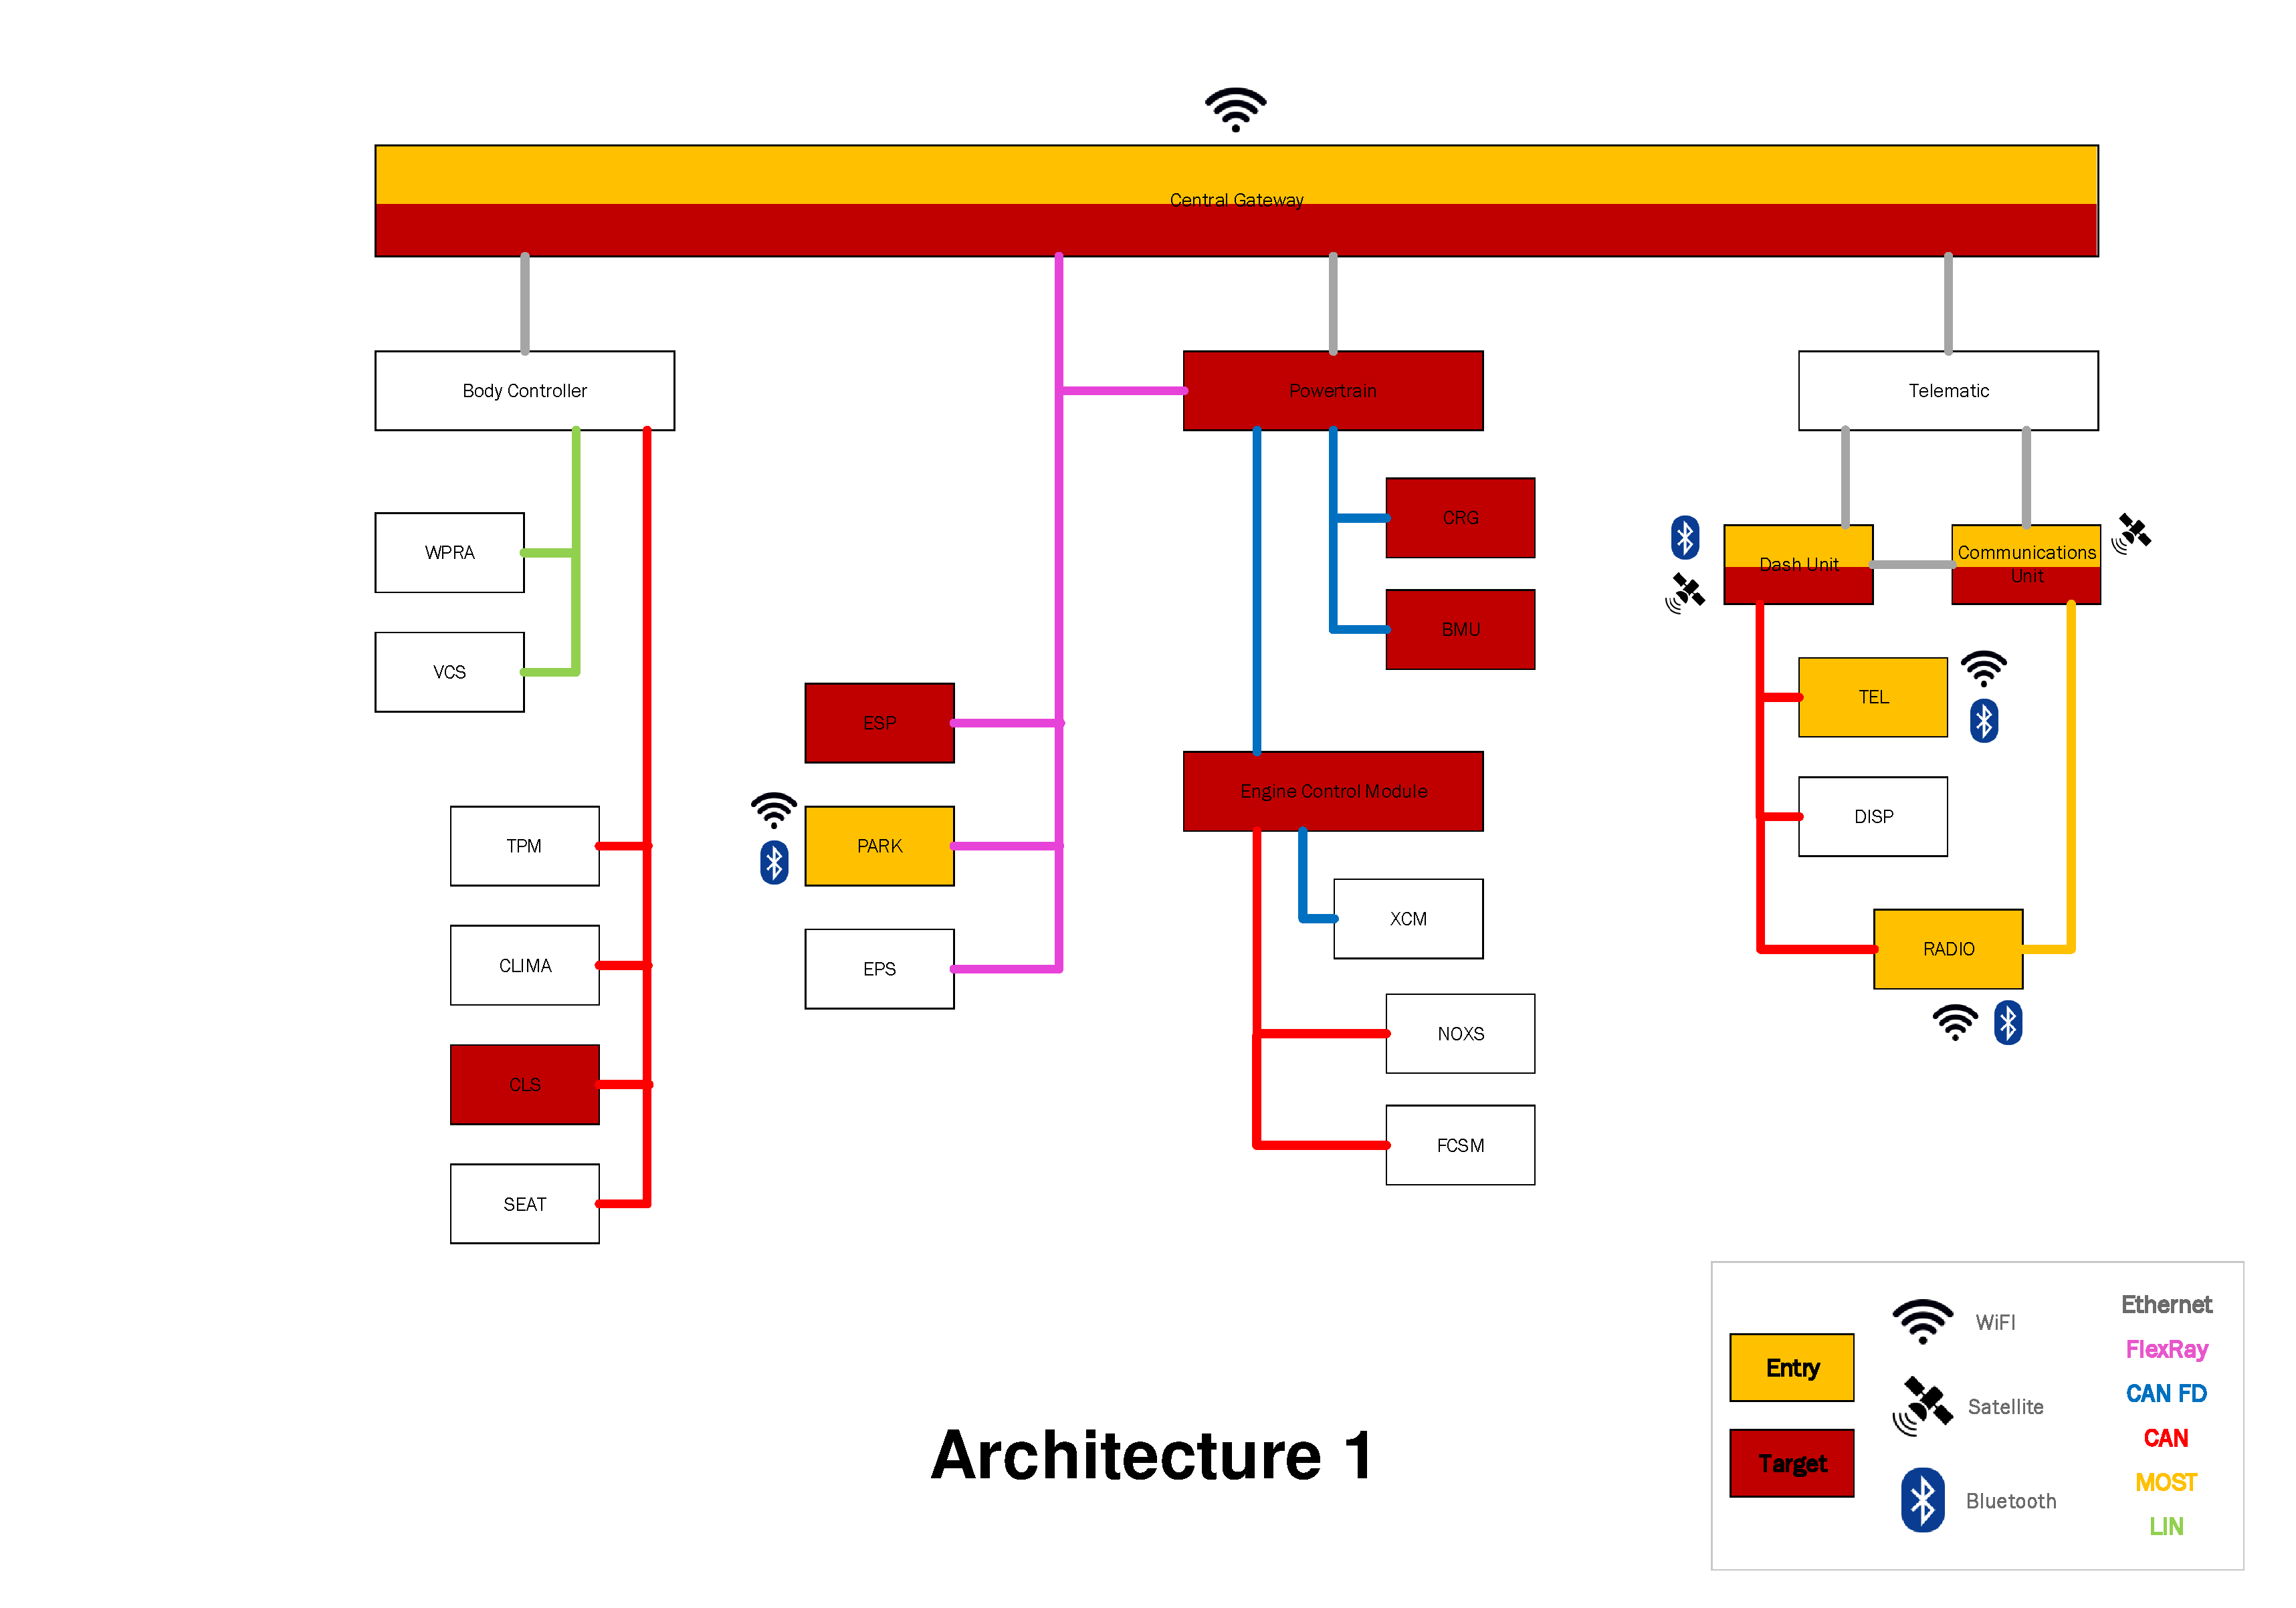
\includegraphics[width=\textwidth, page=1]{../Architectures-survey.pdf}
\end{figure}

\begin{figure}
    \caption{Architecture 2}
    \includegraphics[width=\textwidth, page=2]{../Architectures-survey.pdf}
\end{figure}

\begin{figure}
    \caption{Architecture 3}
    \includegraphics[width=\textwidth, page=3]{../Architectures-survey.pdf}
\end{figure}

\begin{figure}
    \caption{Architecture 4}
    \includegraphics[width=\textwidth, page=4]{../Architectures-survey.pdf}
\end{figure}

\begin{figure}
    \caption{Architecture 5}
    \includegraphics[width=\textwidth, page=5]{../Architectures-survey.pdf}
\end{figure}

\begin{figure}
    \caption{Architecture 6}
    \includegraphics[width=\textwidth, page=6]{../Architectures-survey.pdf}
\end{figure}

\begin{figure}
    \caption{Architecture 7}
    \includegraphics[width=\textwidth, page=7]{../Architectures-survey.pdf}
\end{figure}

\begin{figure}
    \caption{Architecture 8}
    \includegraphics[width=\textwidth, page=8]{../Architectures-survey.pdf}
\end{figure}

\begin{figure}
    \caption{Architecture 9}
    \includegraphics[width=\textwidth, page=9]{../Architectures-survey.pdf}
\end{figure}

\begin{figure}
    \caption{Architecture 10}
    \includegraphics[width=\textwidth, page=10]{../Architectures-survey.pdf}
\end{figure}


\chapter{Deciding on the criteria}
\label{chp:criteria}

One of the most important asepcts of this thesis is the criteria used to evaluate the different architectures.

In order to find and calibrate a good criteria, a survey was conducted in which ten architectures were evaluated by security experts in the field of automotive security.
Their rating and feedback on this "training set" was used to calibrate the criteria used on the main architectures in this thesis.
Doing a survey with such a set rather than the architectures themselves was done to avoid biasing the results, as well as have a well evaluated criteria.
In addition, the training set is much larger than the main set, thus the results are more accurate.

\section{Survey}
\label{sec:survey}

Security experts at Mercedes-Benz Tech Innovation were given ten architectures as shown in \ref{chp:arch}.
The experts were asked to rank the architectures and give reasoning behind their ranking, as well as add any comments they had.
Since there are ten architectures, the ranking went from 1 to 10, where 1 is the most secure and 10 is the least secure.
To get to a result in the end, each rank was given a score, where 1 got 1 points, 2 got 2 points, and so on.
In the end, each ranking or score each architecture got was summed up, and the architecture with the lowest score was the most secure.

The result is as follows:

\begin{table}[h]
    \centering
    \caption{Rank and Architecture}
    \begin{tabular}{ |c|c| } 
    \hline
    Rank & Architecture \\
    \hline
    1 & \ref{subsec:arch3} 3\\
    2 & \ref{subsec:arch8} 8\\
    3 & \ref{subsec:arch6} 6\\
    4 & \ref{subsec:arch10} 10\\
    5 & \ref{subsec:arch2} 2\\
    6 & \ref{subsec:arch7} 1\\
    7 & \ref{subsec:arch1} 5\\
    8 & \ref{subsec:arch9} 7\\
    9 & \ref{subsec:arch5} 9\\
    10 & \ref{subsec:arch4} 4\\
    \hline
    \end{tabular}
\end{table}

Looking at the reason behind the ranking, the experts gave the following feedback:\\

They all agreed that one of the most important criteria is the amount of hops there is between the entry and target.
Hops play a crucial role in an attack path since the more hops there are, the more difficult it is for an attacker to get from entry to target.
However, not every one hop is equal.

One thing that was not considered in these architectures was the security mechanisms implemented in the vehicle, such as firewalls or IDCs.
As already mentioned, they are implicitly considered in the attack feasibility of each component, 
but it has not been specifically stated which ECUs have which security properties.
Security mechanisms, of course, hinder the attacker from progressing quickly through the attack path.

Another aspect are intelligent domain controllers. 
There is a difference whether the domain controller differentiates between the different domains, or if it just forwards messages.

It is of course important to consider them when evaluating the architectures, however in this thesis, 
they are represented through the feasibility of each ECU, bus and interface as mentioned in \ref{sec:config}.

Another crucial factor is isolation - isolation of domains as well as the ECUs themselves, and especially an isolated Powertrain domain.
It gives the opportunity to compartmentalize the system, and security mechanisms can be applied to each domain or ECU individually.
The Powertain domain is the "heart" of the vehicle because it controls the engine, transmission, and other important systems, thus it is crucial to isolate it.
However, it is also not feasibile to have too much isolation, as it would make the system too complex.
For example, Architectures 6 (\ref{subsec:arch6}) and 7 (\ref{subsec:arch7}) are very isolated, but they are also very complex and unfeasible.

Communication between the ECUs must also be considered, as it is a crucial part of the vehicle itself. 
Too many isolated ECUs communicating with each other can lead to a lot of overhead.\\
Media change is also to be considered. 
For example, if a message is sent over CAN, converting it to CANFD is no problem but a different media such as FlexRay or Ethernet requires overhead as well.\\

Other factors include whether a \textit{Central Gateway} is present, which is always beneficial, as well as the amount of external interfaces.
More external interfaces means more attack vectors, and thus more security mechanisms must be implemented.\\

All of these factors result in one hop not being the same as another and thus the hop's properties must be considered when evaluating the architectures.

\section{Criteria}

Having the result from the survey, the criteria used to evaluate the architectures was calibrated.
The amount of hops between the entry and target being the most important criteria, each attack path feasibility is divided by the amount of hops it took from entry to target.
This way, the more hops there are, the less feasible the attack path is.
\chapter{Comparison and Evaluation}
\label{chp:compeval}

This chapter will compare the three main architectures based on the criteria described in \ref{chp:criteria}.


\chapter{Conclusion}
\label{chp:conclusion}

Of course, there is room for improvement.
For exapmle, the security mechanisms implemented in the vehicle, such as firewalls or IDCs, were not considered in great detail, but just as the feasibility of each component.
A more fine granular analysis of each component would be beneficial. This way, you would have to consider more variables and thus get a more accurate result.
However, considering them in this thesis would have made it too complex and too long, and thus it was not done.


\backmatter
\printbibliography[heading=bibintoc]
\printglossary[type=\acronymtype]
\printglossary

\end{document}
